\subsection{Doppler Cooling}
From the form of the dissipative force
\begin{equation}
    F_{dis} = 2\hbar|\Omega|^2 \Vec{k}\frac{\gamma_{21}}{\gamma_{21}^2 + \delta^2},
\end{equation}
we can see the dissipative force not necessarily cools the atoms, it only injects momentum $\hbar\Vec{k}$ at the optical pumping rate. To cool atoms down in one direction, there needs to be a pair of counter-propagating optical fields, and the total dissipative force needs to slow down high speed atoms at a higher rate than to speedup low speed atoms.

\begin{figure}[htbp]
    \centering
    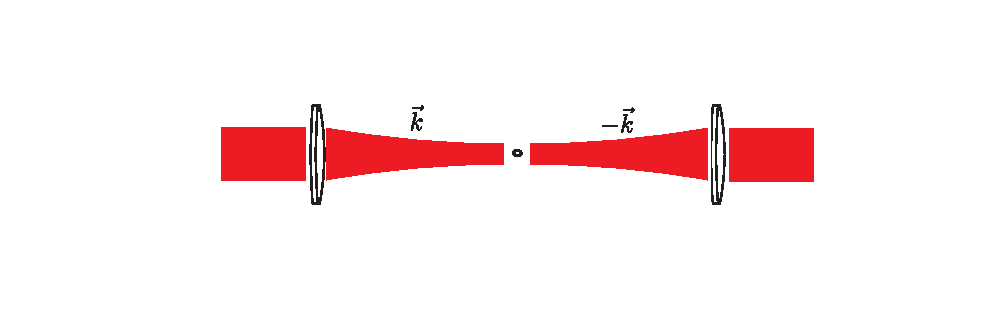
\includegraphics[width=\textwidth]{Chapter2_secs/DopplerCooling.pdf}
    \caption{1D Doppler Cooling. }
    \label{fig:DC}
\end{figure}

When we account for the motion of atoms, Doppler effect shifts the resonance and deuning. With adjusted detuning, the dissipative force takes the form
\begin{equation}
    F_{dis} = 2\hbar|\Omega|^2 \Vec{k}\frac{\gamma_{21}}{\gamma_{21}^2 + (\delta-\Vec{k}\cdot\Vec{v})^2}.
\end{equation}
When the speed of atoms is small, $\Vec{k}\cdot\Vec{v} \ll \delta, \gamma$, we expand the force to the first order of $\Vec{k}\cdot\Vec{v}$,
\begin{equation}
    F_{dis} \approx 2\hbar|\Omega|^2 \Vec{k}\frac{\gamma_{21}}{\gamma_{21}^2 + \delta^2} \left(1 + \frac{2\delta\Vec{k}\cdot\Vec{v}}{\gamma_{21}^2 + \delta^2}\right).
\end{equation}
The total force of A pair of counter-propagating beams cancels the first term and retains the velocity dependent cooling force
\begin{equation}
    F_{tot} = \frac{8\hbar|\Omega|^2\gamma_{21}\delta k^2 v}{(\gamma_{21}^2 + \delta^2)^2}.
\end{equation}

The direction of the force depends on the sign of $\delta$, when $\delta<0$, the force is in the opposite direction of $v$ and acts as a cooling force. When $\delta>0$, the force heats the atoms up with a positive feedback mechanism. Intuitively, the cooling mechanism can be understood from the dependence of optical pumping rate on the Doppler shift. When the light is red detuned, the atoms are closer to resonance with the light beam propagating in the opposite direction from the atoms' velocity. The optical pumping rate of this beam is thus higher than the other, so on the average, the atoms absorbs more photons from this beam and acquires a negative momentum. 

The dissipative force applies to one dimensional cooling, and to the first order of $\Vec{k}\cdot\Vec{v}$, the force is decoupled in different spatial directions. To cool down atoms in all three spatial directions, three pairs of counter-propagating red-detuned light are needed. This is the simplified version of Optical molasses \cite{lett1989optical,ungar1989optical,weiss1989optical}.  Fig.~(\ref{fig:OM}) is the Fig.~(13) in \cite{lett1989optical}, it is the sketch of one of the first experiment of Optical Molasses conducted in NIST, Gaitherburg. The result of the experiment demonstrated the cooling limit of Optical Molasses is well below the limit of Doppler cooling. The explanation requires multi-level system and circular polarized cooling light which is discussed in the Doppler cooling limit and sub-Doppler cooling section.

\begin{figure}[htbp]
    \centering
    \includegraphics[width=\textwidth]{Chapter2_secs/optical_molasses.png}
    \caption{Fig.~(13) in \cite{lett1989optical}, the sketch of the experimental appartus of Optical Molasses experiment. }
    \label{fig:OM}
\end{figure}